\mode*

\begin{frame}
  \tableofcontents
\end{frame}


\section[Book and author]{The book and author}

\begin{frame}
  \begin{figure}
    
\includegraphics[height=0.8\textheight]{fig/book.jpg}
    \caption{Front cover of Necessary Conditions of Learning.}
  \end{figure}
\end{frame}

\begin{frame}
  \begin{figure}
    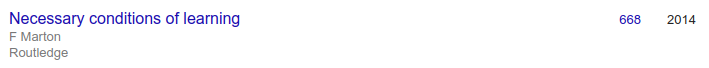
\includegraphics[width=\columnwidth]{fig/necessary-conditions-citations.png}
    \caption{Citations for the book.}
  \end{figure}
\end{frame}

\begin{frame}
  \begin{figure}
    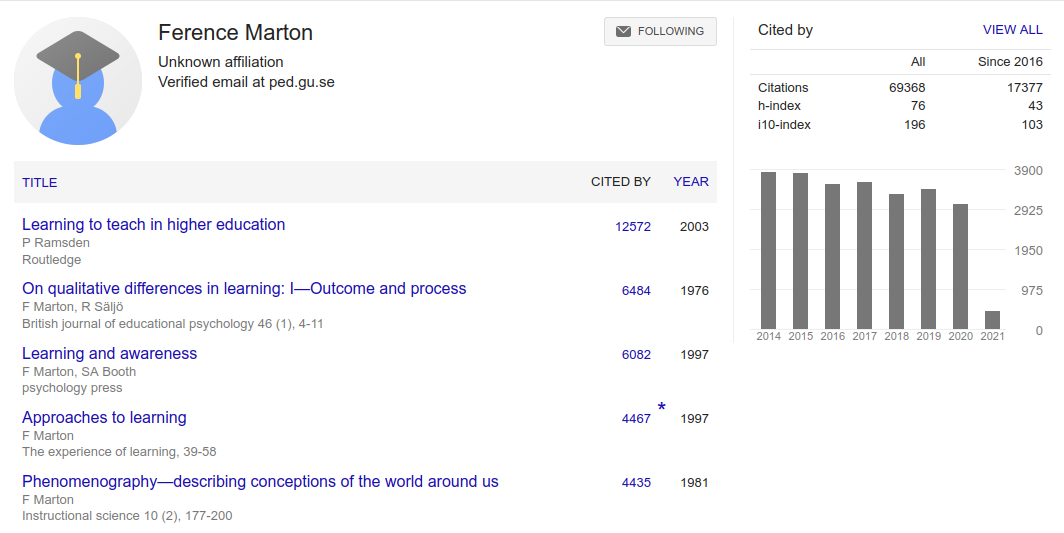
\includegraphics[width=\columnwidth]{fig/marton-gscholar.png}
    \caption{Marton's profile on Google Scholar, showing his high citation 
    counts.}
  \end{figure}
\end{frame}

\begin{frame}
  \textcquote[p.~210]{NecessaryConditionsOfLearning}{%
    \textins{T}he particular theory in this book is not about the general 
    aspects but about the specific aspects (\ie, those related to the content 
    of learning).
    Most other theories of learning are about the general aspects.
    This one is not, except when learning is learning to learn.%
  }
\end{frame}

\begin{frame}
  \begin{block}{Main ideas}
    \begin{itemize}
      \item Phenomenography~\cite{Phenomenography}
      \item Variation theory~\cite{VariationTheory}
      \item Learning studies~\cite{LearningStudy}
    \end{itemize}
  \end{block}
\end{frame}


\section{Phenomenography}

\begin{frame}
  \blockcquote{NecessaryConditionsOfLearning}{%
    We tacitly assume that what we see is exactly what is there to be seen and 
    that others see things in the same way we do. It is hard to realize that we 
    have actually learned to see the world in certain ways and that others may 
    have learned to see it differently.
  }
\end{frame}

\begin{frame}
  \begin{block}<1-2>{Phenomenography~\cite{Phenomenography}}
    \begin{itemize}
      \item Reality is experienced.
      \item People interpret significant aspects of reality.
    \end{itemize}
    \pause
    \begin{description}
      \item[First-order perspective] describes various aspects of the world.
      \item[Second-order perspective] describes people's experiences of various 
        aspects of the world --- phenomenography.
    \end{description}
  \end{block}
\end{frame}


\section{Variation theory}

\begin{frame}
  \begin{block}{Variation theory~\cite{VariationTheory}}
    \vspace{-0.5em}
    \[
      \text{learning}
      \quad\leftarrow\quad
      \text{discernment}
      \quad\leftarrow\quad
      \text{variation}
    \]
  \end{block}

  \pause

  \begin{remark}
    \begin{itemize}
      \item There must be a pattern of variation to experience.
      \item \emph{This pattern must be experienced}.
    \end{itemize}
  \end{remark}
\end{frame}

\begin{frame}
  \begin{block}{Patterns of variation}
    \vspace{-0.5em}
    \[
      \text{contrast}
      \quad\rightarrow\quad
      \text{generalization}
      \quad\rightarrow\quad
      \text{fusion}
    \]
  \end{block}

  \begin{figure}
    \begin{subfigure}{0.3\columnwidth}
      \centering
      \includegraphics{fig/contrast-color.tikz}
      \caption{Contrast}
    \end{subfigure}
    \hfill
    \begin{subfigure}{0.3\columnwidth}
      \centering
      \includegraphics{fig/generalization-color.tikz}
      \caption{Generalization}
    \end{subfigure}
    \hfill
    \begin{subfigure}{0.3\columnwidth}
      \centering
      \includegraphics{fig/fusion-color.tikz}
      \caption{Fusion}
    \end{subfigure}
    \caption{%
      Illustrating the patterns of variation for aspects color and shape.
    }
  \end{figure}
\end{frame}

\begin{frame}
  \begin{figure}
    \semitransp{%
      \begin{subfigure}{0.3\columnwidth}
        \centering
        \includegraphics{fig/contrast-color.tikz}
        \caption{Contrast}
      \end{subfigure}
    }
    \hfill
    \begin{subfigure}{0.3\columnwidth}
      \centering
      \includegraphics{fig/generalization-color.tikz}
      \caption{Generalization}
    \end{subfigure}
    \hfill
    \semitransp{%
      \begin{subfigure}{0.3\columnwidth}
        \centering
        \includegraphics{fig/fusion-color.tikz}
        \caption{Fusion}
      \end{subfigure}
      \caption{%
        Illustrating the patterns of variation for aspects color and shape.
      }
    }
  \end{figure}

  \begin{remark}
    \begin{itemize}
      \item We tend to focus on induction (\ie generalization without 
        contrast).
      \item \enquote{Good theses from previous years.}
      \item \enquote{One example of linear function, another example of linear 
        function.}
    \end{itemize}
  \end{remark}
\end{frame}


\section{Learning study}

\begin{frame}
  \begin{block}{Learning study~\cite{LearningStudy}}
    \begin{itemize}
      \item Design-Based Research + Variation Theory
      \item Extends the Japanese concept Lesson Study.
    \end{itemize}
    \pause
    \begin{enumerate}
      \item \label{design} (Re-)Design teaching material/plan using variation 
        theory.
      \item Perform teaching.
      \item Analyze teaching performance and student outcomes.
      \item Go to \ref{design}.
    \end{enumerate}
  \end{block}

  \pause

  \begin{remark}
    \begin{itemize}
      \item Teacher teams, teach the same thing to different classes.
      \item Yields iterations.
    \end{itemize}
  \end{remark}
\end{frame}

\begin{frame}
  \begin{example}
    \begin{itemize}
      \item I'll work systematically according to this with my TAs.
      \item Review the main material and labs (weekly modules).
      \item Two TAs, two non-parallel tutorial groups.
    \end{itemize}
  \end{example}
\end{frame}


\section{Disposition}

\begin{frame}
  \begin{enumerate}
    \item \textbf<2>{What makes humans human?}
      \hfill
      \onslide<2>{(forms of learning)}
    \item \textbf<3>{What is to be learned?}
      \hfill
      \onslide<3>{(learning objectives)}
    \item \textbf<4>{Sameness and difference in learning}
      \hfill
      \onslide<4>{(variation theory)}
    \item \textbf<5>{What does the world look like to others?}
      \hfill
      \onslide<5>{(phenomenography)}
      \setcounter{chnum}{\value{enumi}}
  \end{enumerate}
  \begin{enumerate}
    \setcounter{enumi}{\value{chnum}}
    \item \textbf<6>{The art of learning}
      \hfill
      \onslide<6>{(learning alone, doing research)}
    \item \textbf<7>{Making learning possible}
      \hfill
      \onslide<7>{(teaching)}
    \item \textbf<8>{Learning to help others to learn}
      \hfill
      \onslide<8>{(education research)}
  \end{enumerate}
\end{frame}

